% %%%%%%%%%%%%%%%%%%%%%%%%%%%%%%%%%%%%%%%%%%%%%%%%%%%%%%%%%%%%%%%%%%%%%
% %% Theory %%
% C Model
% %%%%%%%%%%%%%%%%%%%%%%%%%%%%%%%%%%%%%%%%%%%%%%%%%%%%%%%%%%%%%%%%%%%%%

\section{Model for Reduction Cache}
\label{sec:theory:cmodel}

\lettrine{T}{o} go beyond simply observing the behavior of a specific accelerator processing a given matrix, a model of the matrix and the cache is required.
We present a hybrid probabilistic/fast simulation model for a \gls{redC}, processing \acrshort{op} \acrshort{spmv}, which predicts the volume of memory traffic issued by the L1 cache, starting from a matrix density distribution and a cache configuration.

The model represents the non-zero density both in the matrix and in the cache, with cache-line granularity.
Using these coarse grain densities, a fast simulation of the \acrshort{op} \acrshort{spmv} is performed.
The state of the cache can be predicted at each step of the simulation.
By counting the \glspl{eviction}, we evaluate the output memory traffic, the memory trafic of the output vector $c$.
We can thus predict the total number of memory accesses for different types of matrices and quickly explore different \gls{redC} configurations.

We do not consider the sequential accesses to the input matrix $A$ and vector $b$ in our model.
Indeed, the matrix tables $\mathit{val}$, $\mathit{idx}$ and $\mathit{ptr}$, and the vector $b$ are each read once, giving a total memory traffic of $2\mathit{nnz} + (M+1) + M$ elements.
We showed in previous section that a simple generic cache of reasonable size is enough to handle the inputs.

Our model uses the cache configuration parameters $S$, $W$ and $l$.
Although our model is not limited to \gls{banded} matrices, they are the focus of this work.
The matrix density distribution thus takes on two different values, either $d_\mathit{IB}$ in the band, or $d_\mathit{OB}$ outside of the band.

We normalize the memory traffic by dividing the number of elements that are read or written by the number of non-zero elements ($nnz$) in the matrix, so we can compare performance between matrices of different sizes and densities.
Indeed, we can interpret the normalized memory traffic, $\mathit{normMT}$, as the number of elements transferred from/to memory per non-zero matrix element.
If the memory traffic remains constant while the matrix density increases, we expect $\mathit{normMT}$ to decrease.

% %%%%%%%%%%%%%%%%%%%%%%%%%%%%%%%%%%%%%%%%%%%%%%%%%%%%%%%%%%%%%%%%%%%%%
\subsection{Operation of the Analytical Model}
\label{sec:theory:model}

\paragraph{Matrix Representation}
The square matrix is of dimension $M$, as represented in Figure~\ref{fig:theory:model:matrix_cache_rep}.
Its rows and columns are indexed by $0 \leqslant i, j \leqslant M-1 \in \mathbb{N}$.
Each column is split into vertical-strips of size $l$, where $l$ is the cache-line size.
Indeed a vertical-strip is a portion of a column $j$ of size $l$, from row-indices $i$ to $i+l-1$, as illustrated by the \textit{red} rectangle within the matrix in the figure.
Within a column, vertical-strips are indexed by $k \in \ldb0, M_l-1\rdb$~\footnote{We use $\ldb a, b\rdb$ for the integer intervals, and $[a, b]$ for real intervals.}, with $M_l = \left\lceil\frac{M}{l}\right\rceil$, and $k = \left\lceil\frac{i}{l}\right\rceil$.

The matrix is thus represented as a static, dense two dimensional table, $\mathit{MDT}$ (\textit{Matrix Density Table}), of size $(M_l, M)$ that contains the density in $[0, 1]$ of each vertical-strip.
We assume that the distribution of the non-zero elements within a vertical-strip is uniform, as assumed in related work~\cite{Temam1992_Model} where the authors studied a directly-mapped generic cache for an \acrlong{ip} \acrshort{spmv} kernel, only for the case of \gls{PBanded} matrices.

\begin{figure}[htbp]
    \centering
    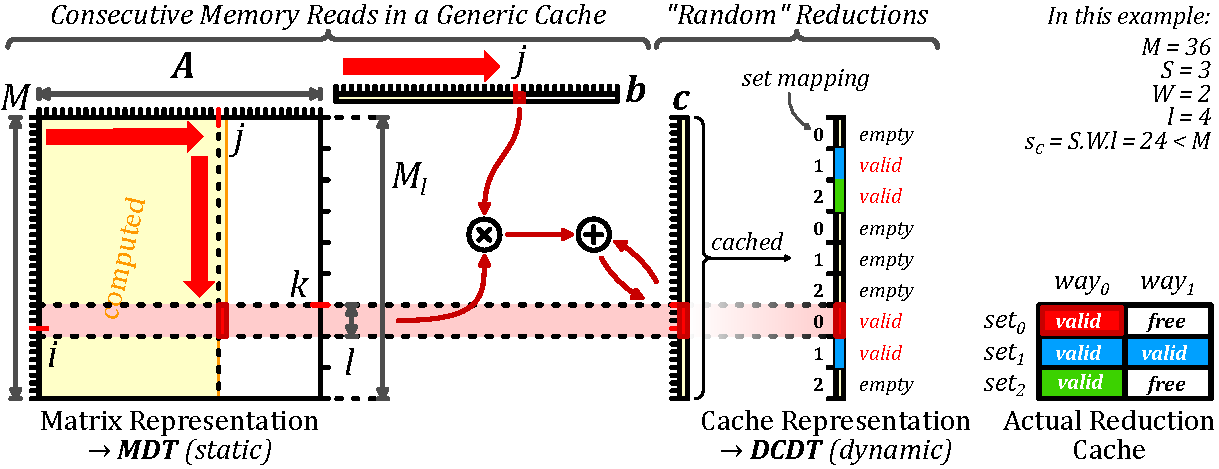
\includegraphics[width=\linewidth]{Chapter_Theory/Figures/PDF/CModel_Mat&Cache_Rep.pdf}
    \caption{Input Matrix and Cache Representation of the Model}
    \label{fig:theory:model:matrix_cache_rep}
\end{figure}

\paragraph{Cache Representation}
Still in Figure~\ref{fig:theory:model:matrix_cache_rep}, the cache is represented as a single column, which maps directly to the output vector $c$.
This ``column-representation'' of the cache is partitioned into cache-lines, corresponding directly to the vertical-strips of a given column of the matrix, as shown by the horizontal \textit{light red} rectangle.
A cache-line $k \in \ldb0, M_l-1\rdb$ is stored in a unique \gls{set} $s \in \ldb0,S-1\rdb$ of the cache such that $s = k \% S$.
Unlike the matrix representation which is static, the cache representation is continuously updated as the model evaluates \acrshort{op} \acrshort{spmv}.

Of course, the real cache-size ($S \times W \times l$) is not necessarily equal to the output vector size ($M$).
Thus, at a given time, the number of valid (non-empty) cache-lines contained in the cache representation must not exceed the actual cache-size.
Specifically, we ensure the number of valid cache-lines in a \gls{set} of the cache representation does not exceed the number of ways $W$.
In the example in Figure~\ref{fig:theory:model:matrix_cache_rep}, the actual cache is holding four valid cache-lines, which are the only valid cache-lines present in the cache representation.

To count the number of valid cache-lines, we further distinguish them from empty ones.
For this reason, we set the cache-line densities to be either zero (the cache-line is empty), or the density is in the range $\left[\frac{1}{l}, 1\right]$ (the cache-line is valid).
A valid cache-line has a density between $\frac{1}{l}$ and $1$, corresponding to the probabilistic number of non-zero elements.

The state of the cache is thus represented with the dynamic table $\mathit{DCDT}$ (\textit{Disjoint Cache Density Table}), of dimension $M_l$ that contains the disjoint-density in $\{0\} \cup \left[\frac{1}{l}, 1\right]$ of each cache-line, at a given iteration.
Initially, all cache-lines are set to zero density, since the cache is considered empty.

\paragraph{Iterative Process}
In the fast simulation phase, the analytical model~\cite{FRIEDENTHAL2012_AnalyticalModel} iterates over the vertical-strips in the matrix, following the dense traversal of the \acrshort{op} algorithm, as described in Chapter~\ref{cha:background} and shown with \textit{red} arrows in Figure~\ref{fig:theory:model:matrix_cache_rep}.
In a given iteration (column $j$, vertical-strip $\kappa$), we use the matrix density of the current vertical-strip, $\mathit{MDT}_{\kappa,j}$, and the current state of $\mathit{DCDT}$ to determine if an \gls{eviction} occurs, and update it for the next iteration, if necessary.

\paragraph{Disjoint-Density of the Current Vertical-Strip}
The density of the current vertical-strip in the matrix has to be disjointed at each iteration, to determine whether the strip is empty or not, as done for the cache-lines.
We define the vertical-strip disjoint-density as $d_\mathit{lM}(\kappa) \in \{0\} \cup [\frac{1}{l}, 1]$.
\begin{itemize}
    \item When $\mathit{MDT}_{\kappa,j} = 0$, the vertical-strip in the matrix is empty, thus, $d_\mathit{lM}(\kappa) = 0$.
    \item When $0 < \mathit{MDT}_{\kappa,j} < \frac{1}{l}$, the vertical-strip can have either $0$ or $1$ non-zero elements.
            To resolve this, we maintain a running counter of the accumulated $\mathit{MDT}_{\kappa,j}$ values, and when this counter exceeds $\frac{1}{l}$, the current vertical-strip is considered non-empty, so we set $d_\mathit{lM}(\kappa) = \frac{1}{l}$.
            If the counter is below this threshold, $d_\mathit{lM}(\kappa) = 0$.
            %To avoid undesired aliasing artifacts, we add a small random variation to this threshold.
    \item When $\mathit{MDT}_{\kappa,j} \geqslant \frac{1}{l}$, the vertical-strip has one or several non-zero elements.
          Thus, $d_\mathit{lM}(\kappa) = \mathit{MDT}_{\kappa,j}$.
\end{itemize}

With this definition, we can distinguish empty ($d_\mathit{lM}(\kappa) = 0$) and non-empty ($d_\mathit{lM}(\kappa) \ne 0$) vertical-strips.

\paragraph{Eviction Processing}
With the above definitions, we can determine if a \gls{miss} occurs at the current iteration.
A \gls{miss} occurs when the cache-line $\kappa$ is not valid and the vertical-strip is not empty.
Recall that in a \gls{redC}, a \gls{miss} without \gls{eviction} results in the allocation of a free cache-line, initially filled with zeros, and produces no memory traffic.
We define \mbox{$\mathit{miss}(\kappa) = (\mathit{DCDT}_\kappa = 0) \; and \; (d_\mathit{lM}(\kappa) \ne 0)$}, a boolean indicating whether a \gls{miss} occurs in the current iteration.

When allocating a free cache-line, it is necessary to ensure that the number of valid cache-lines in the \gls{set} \mbox{$s = \kappa \% S \in \ldb0,S-1\rdb$} does not exceed $W$.
The new allocation may thus trigger an \gls{eviction}.
Stated formally, $\mathit{nnzcl}_\kappa$ is the count of the cache-lines $k$ from the \gls{set} $s$ that verify $\mathit{DCDT}_k \ne 0$.
We define \mbox{$\mathit{evict}(\kappa) = \mathit{miss}_\kappa \; and \; (\mathit{nnzcl}_\kappa = W)$}, a boolean indicating whether an \gls{eviction} occurs in the current iteration.

In the case of an \gls{eviction}, for the probabilistic model, we use a \textit{random} \gls{eviction} policy to select a valid cache-line in the \gls{set} $s$ (when $\mathit{DCDT}_k \ne 0$).
The index of the evicted cache-line is $e \in \ldb0, M_l-1\rdb$.

\paragraph{Cache Update}
The last step is to update $\mathit{DCDT}$ before proceeding to the next iteration.
(1) If a cache-line is evicted, we must account for the memory traffic and reset the victim line $e$;
(2) The density of the current cache-line $\kappa$ may increase if there is a \gls{hit} or if it is newly allocated:
\begin{enumerate}
    \item In the case of an \gls{eviction} ($\mathit{evict}(\kappa)$ is true), we reset the victim cache-line ($e$) by setting $\mathit{DCDT}_e = 0$.
    \item We update the density of the cache-line $\kappa$.
    In the case of a \gls{miss} ($\mathit{DCDT}_\kappa = 0$), the cache-line density is set to the disjoint-density of the matrix vertical-strip $\kappa$.
    In the case of a \gls{hit}, the cache-line and the vertical-strip densities are merged: \\
    $\mathit{DCDT}_\kappa \gets \mathit{DCDT}_\kappa + (1 - \mathit{DCDT}_\kappa) \times d_\mathit{lM}(\kappa)$
\end{enumerate}
The updated cache-line density is either $0$ or greater than $\frac{1}{l}$, thus respecting the constraint that the cache-line is either empty or valid.

\paragraph{Final Iteration}
Starting with an initially empty cache, we run all $M \times M_l$ iterations and count the total number of \glspl{eviction} ($\mathit{nbEvict}$).
After the last iteration, we account for the memory transactions required to flush the cache ($\mathit{nbFlush}$), writing the valid cache-lines to memory, by counting lines where $\mathit{DCDT}_k \ne 0$, for $k \in \ldb0, M_l-1\rdb$.
$\mathit{nbFlush}$ will never exceed \mbox{$S \times W$}.

In a \gls{redC}, \glspl{eviction} and flushes result in a line-wise memory read, a modification, and a line-wise memory write.
The update memory traffic is $2 l (\mathit{nbEvict} + \mathit{nbFlush})$ elements, and $\mathit{normMT}$ is this amount divided by $nnz$.

\begin{highlight}{Conclusion}{Red}
    We have presented a \textbf{hybrid probabilistic/fast simulation analytical model} for a \gls{redC}, processing \acrshort{op} \acrshort{spmv}, which predicts the volume of memory traffic issued by the L1 cache, starting from a \textbf{matrix density distribution} and a \textbf{cache configuration}.
    The model represents the non-zero density both in the matrix and in the cache, with \textbf{cache-line granularity}.
    Using these coarse grain densities, a \textbf{fast simulation} of the \acrshort{op} \acrshort{spmv} is performed.
    In this way, we can quickly explore different \gls{redC} configurations to evaluate their impact on memory traffic.
    % In this way, we can quickly explore different \gls{redC} configurations and matrix types to evaluate their impact on memory traffic.
\end{highlight}